\documentclass[12pt]{article}
\usepackage{graphicx}
\usepackage{placeins}


% acronyms for text or math mode
\newcommand {\ccast} {\mbox{\small CCAST}}
\newcommand {\cris} {\mbox{\small CrIS}}

\newcommand {\airs} {\mbox{\small AIRS}}
\newcommand {\iasi} {\mbox{\small IASI}}
\newcommand {\idps} {\mbox{\small IDPS}}
\newcommand {\nasa} {\mbox{\small NASA}}
\newcommand {\noaa} {\mbox{\small NOAA}}
\newcommand {\nstar} {\mbox{\small STAR}}
\newcommand {\umbc} {\mbox{\small UMBC}}
\newcommand {\uw}   {\mbox{\small UW}}

\newcommand {\fft}  {\mbox{\small FFT}}
\newcommand {\ifft} {\mbox{\small IFFT}}
\newcommand {\fir}  {\mbox{\small FIR}}
\newcommand {\fov}  {\mbox{\small FOV}}
\newcommand {\for}  {\mbox{\small FOR}}
\newcommand {\ict}  {\mbox{\small ICT}}
\newcommand {\ils}  {\mbox{\small ILS}}
\newcommand {\igm}  {\mbox{\small IGM}}
\newcommand {\opd}  {\mbox{\small OPD}}
\newcommand {\rms}  {\mbox{\small RMS}}
\newcommand {\zpd}  {\mbox{\small ZPD}}
\newcommand {\ppm}  {\mbox{\small PPM}}
\newcommand {\srf}  {\mbox{\small SRF}}
\newcommand {\sdr}  {\mbox{\small SDR}}

\newcommand {\ES} {\mbox{\small ES}}
\newcommand {\SP} {\mbox{\small SP}}
\newcommand {\IT} {\mbox{\small IT}}
\newcommand {\SA} {\mbox{\small SA}}

\newcommand {\ET} {\mbox{\small ET}}
\newcommand {\FT} {\mbox{\small FT}}

\newcommand {\wn} {\mbox{cm$^{-1}$}}

% abbreviations, mainly for math mode
\newcommand {\real} {\mbox{real}}
\newcommand {\imag} {\mbox{imag}}
\newcommand {\atan} {\mbox{atan}}
\newcommand {\obs}  {\mbox{obs}}
\newcommand {\calc} {\mbox{calc}}
\newcommand {\sinc} {\mbox{sinc}}
\newcommand {\psinc} {\mbox{psinc}}
\newcommand {\std} {\mbox{std}}

% symbols, for math mode only
\newcommand {\lmax} {L_{\mbox{\tiny max}}}
\newcommand {\vmax} {V_{\mbox{\tiny max}}}

\newcommand {\tauobs} {\tau_{\mbox{\tiny obs}}}
\newcommand {\taucal} {\tau_{\mbox{\tiny calc}}}
\newcommand {\Vdc}  {V_{\mbox{\tiny DC}}}

\newcommand {\rIT} {r_{\mbox{\tiny\textsc{ict}}}}
\newcommand {\rES} {r_{\mbox{\tiny\textsc{es}}}}
\newcommand {\robs} {r_{\mbox{\tiny obs}}}

\newcommand {\rITobs} {r_{\mbox{\tiny\textsc{ict}}}^{\mbox{\tiny obs}}}
\newcommand {\rITcal} {r_{\mbox{\tiny\textsc{ict}}}^{\mbox{\tiny cal}}}

\newcommand {\ITmean} {\langle\mbox{\small IT}\rangle}
\newcommand {\SPmean} {\langle\mbox{\small SP}\rangle}


\title{AIRS Deconvolution and Translation \\
  from AIRS to CrIS IR Sounders \\
  \vspace{3mm}
  {****} DRAFT {****}\\
}

\author{Howard E.~Motteler \\
  L.~Larrabee Strow \\
  \\
  UMBC Atmospheric Spectroscopy Lab \\
  Joint Center for Earth Systems Technology \\
}

\date{\today}
\begin{document}
\maketitle

\section{Introduction}

Upwelling infrared radiation as measured by the {\airs}
\cite{airs1}, {\iasi} \cite{iasi1}, and {\cris} \cite{cris1,cris2}
sounders is a significant part of the long term climate record.  We
would like to treat this information as a single data set but the
instruments have different spectral resolutions, channel response
functions, and band spans.  As a significant step in addressing this
problem we consider several channel radiance translations---{\iasi}
to high resolution {\cris}, {\iasi} to {\airs}, {\airs} to standard
resolution {\cris}, and high resolution {\cris} to {\airs}.

Translation from {\airs} to {\cris} presents a special challenge
because {\cris} and {\iasi} are Michaelson interferometers with
parametrized response functions, while {\airs} is a grating
spectrometer with channel center frequencies and individually
tabulated spectral response functions determined by the focal plane
geometery.  In section \ref{decon} we show how to take advantage of
detailed knowledge of the {\airs} spectral response functions (SRFs)
to deconvolve {\airs} channel radiances to a resolution-enhanced
intermediate representation.

The translations presented here are validated by comparison with
calculated reference truth.  For example to test the {\iasi} to
{\airs} translation we start with 49 fitting profiles spanning a
significant range of atmospheric conditions \cite{sarta1,sarta2}.
Upwelling radiance is calculated at a 0.0025 {\wn} grid with kcarta
\cite{kcarta1} over a band spanning the {\airs} and {\iasi} response
functions.  ``True {\airs}'' is calculated from this by convolving
the kcarta radiances with {\airs} SRFs, and ``true {\iasi}'' by
convolving kcarta radiances to the {\iasi} instrument
specifications.  {\iasi} is then translated to {\airs} (we call this
``{\iasi} {\airs}'') and compared with true {\airs}.  This sort of
validation assumes perfect knowledge of the {\airs} and {\iasi}
instrument response functions and so gives only a lower bound on
residuals, and on how well the translations can work in practice.
The better we know the response functions, the closer practical
translations can approach these limits.

The conversions here are presented in order of the size of the
residuals, with {\iasi} to high resolution {\cris} most accurate and
high resolution {\cris} to {\airs} the least.  After the sections on
translation, the {\airs} deconvolution is examined in greater
detail.  This report is the theoretical basis document for the
sounder radiance translations implemented in the airs\_decon and
iasi\_deon git repositories.  In addition to the translations, the
repositories include the test and validation code used to produce
the results shown here.  They are available at github,
\begin{verbatim}
  https://github.com/strow/airs_deconv.git
  https://github.com/strow/iasi_decon.git
\end{verbatim}

\section{AIRS Deconvolution}
\label{decon}

\renewcommand{\vec}[1]{\mathbf{#1}}

\begin{figure}
  \centering
  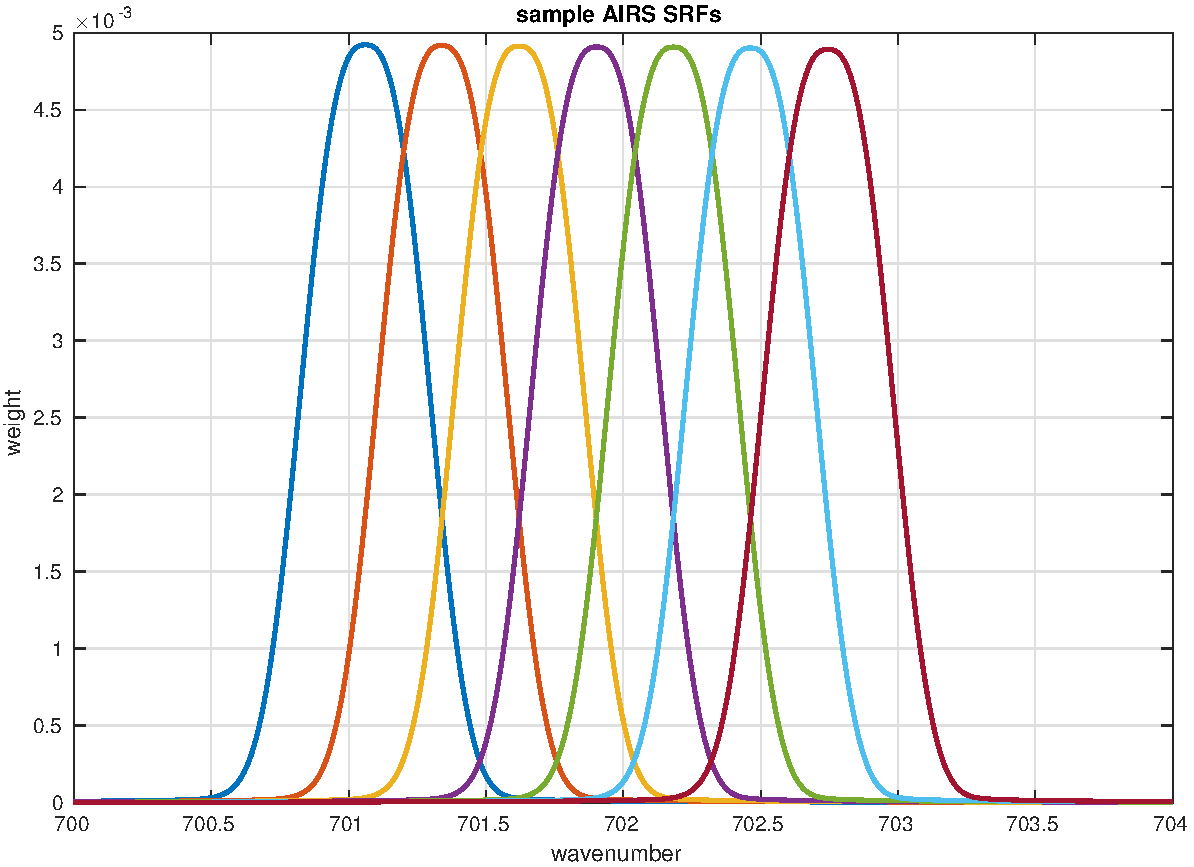
\includegraphics[height=8cm]{figures/airs_sample_SRFs.pdf}
  \caption{sample adjacent {\airs} spectral response functions}
  \label{srfs1}
\end{figure}

\begin{figure}
  \centering
  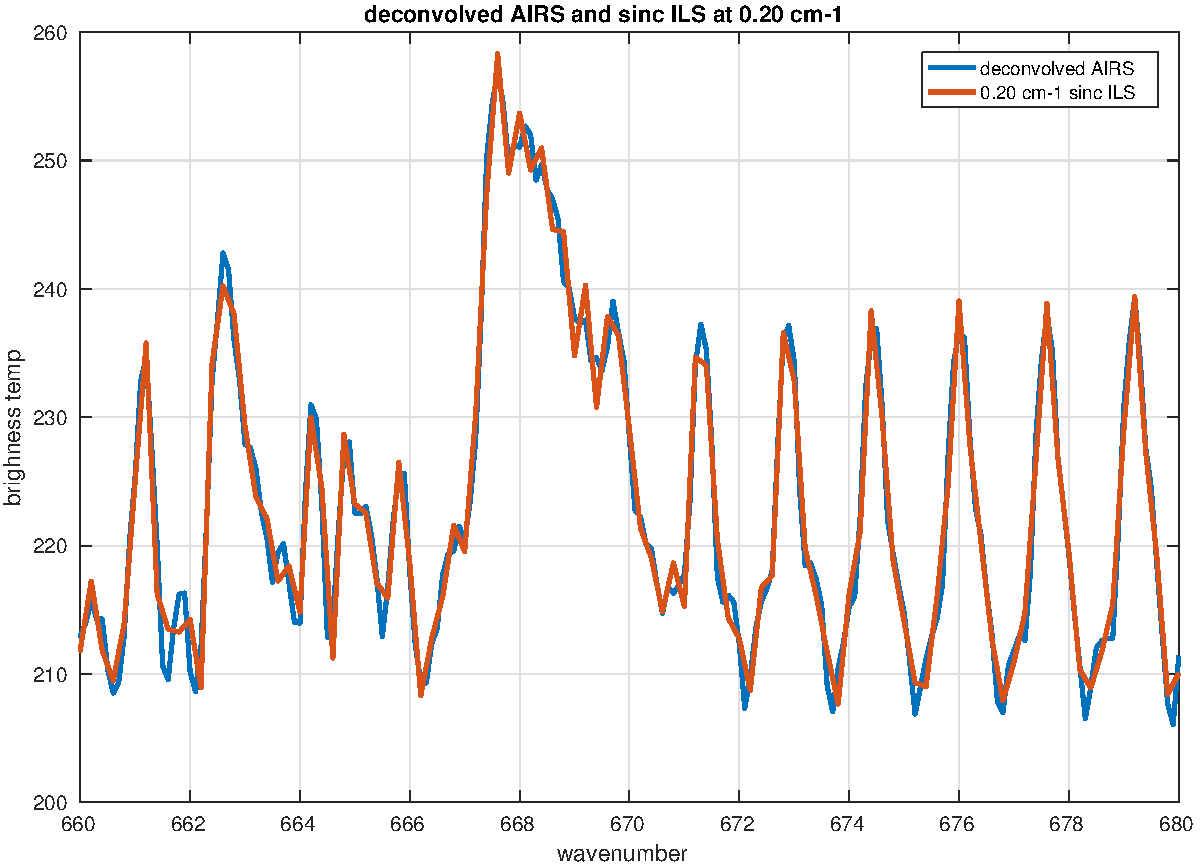
\includegraphics[height=8cm]{figures/airs_decon_res.pdf}
  \caption{deconvolved {\airs} and kcarta 0.0025 {\wn} radiances
    convolved to a sinc ILS at 0.2 {\wn}}
  \label{dsinc}
\end{figure}

\begin{figure}
  \centering
  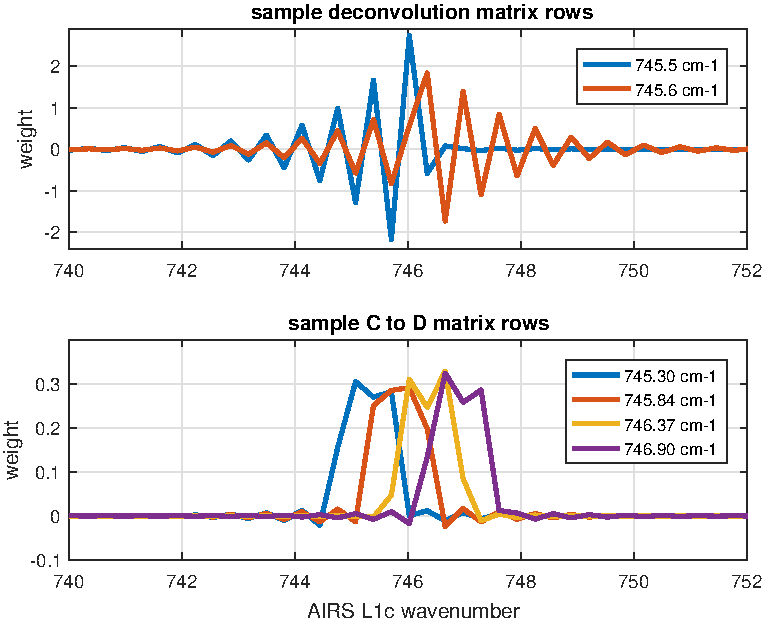
\includegraphics[height=8cm]{figures/airs_decon_basis.pdf}
  \caption{sample basis function for deconvolved {\airs} radiances}
  \label{dbasis}
\end{figure}

The {\airs} spectral response functions model channel response as a
function of frequency and associate channels with nominal center
frequencies.  Each {\airs} channel $i$ has an associated spectral
response function or {\srf} $\sigma_i(v)$ such that the channel
radiance $c_i = \int \sigma_i(v)r(v)\,dv$, where $r$ is radiance at
frequency $v$.  The center or peak of $\sigma_i$ is the nominal
channel frequency.

Figure \ref{srfs1} shows a typical subset of {\airs} SRFs.  Note the
significant overlap in the wings.  This allows the deconvolution to
recover resolution beyond that of the response functions considered
individually.  The spacing of the AIRS L1b channels is not regular;
there are both gaps and close neighbors, side effects of the focal
plane geometry.  Both the gaps and close neighbors cause problems for
a deconvolution.  The AIRS L1c channel set \cite{airs1c} is a derived
product of the 1b set with filled gaps and relatively regular (though
still frequency dependent) frequency spacing, and we will use the 1c
set here.

Suppose we have $n$ channels and a frequency grid $\vec v$ of $k$
points spanning the domains of the functions $\sigma_i$.  The grid
step size for our applications is often 0.0025 {\wn}, the kcarta
resolution.  Let $S_k$ be an $n\times k$ array such that $s_{i,j} =
\sigma_i(v_j)/w_i$, where $w_i = \sum_j \sigma_i(v_j)$, that is
where row $i$ is $\sigma_i(v)$ tabulated at the grid $\vec v$ and
normalized so the row sum is 1.  If the channel centers are in
increasing order $S_k$ is banded, and if they are not too close the
rows are linearly independent.  $S_k$ is a linear transform whose
domain is radiance at the grid $\vec v$ and whose range is channel
radiances.  If $r$ is radiance at the grid $\vec v$, then $c = S_k r$
gives a good approximation of the channel radiances $c_i = 
\int\sigma_i(v)r(v)\,dv$.

In practice this is how we convolve kcarta or other simulated
radiances to get {\airs} channel radiances.  We construct $S_k$
either explicitly or implicitly from {\airs} {\srf} tabulations.
The matrix $S_k$ in the former case is large but manageable with a
banded or sparse representation.

Suppose we have $S_k$ and channel radiances $c$ and want to 
find $r$, that is, to deconvolve $c$.  Consider the linear system
$S_k x = c$.  Since $n < k$ for the kcarta grid mentioned above this
is underdetermined, with infinitely many solutions.  We could add
constraints, take a pseudo-inverse, consider a new matrix $S_b$ with
columns tabulated at some coarser grid, or some combination of the
above.

For an {\airs} to {\cris} translation we are mainly interested in 
the transform $S_b$ with {\srf}s at an intermediate grid, typically
0.1 {\wn}, the approximate resolution of the {\srf} measurements.
Let $\vec v_b = v_1,v_2,\ldots,v_m$ be a 0.1 {\wn} grid spanning the
domains of the functions $\sigma_i$.  Similar to $S_k$, let $S_b$ be
an $n\times m$ array where row $i$ is $\sigma_i(v)$ tabulated at the
$\vec v_b$ grid, with rows normalized to~1.  If $r$ is radiance at
the $\vec v_b$ grid, then $c = S_b r$ is still a reasonable
approximation of $\int\sigma_i(v)r(v)\,dv$.

Consider the linear system $S_b x = c$, similar to the case 
$S_k x = c$ above, where we are given $S_b$ and channel signals $c$
and want to find radiances $x$.  Since $n < m < k$, as with $S_k$
the system will be underdetermined but more manageable because $m$
is approximately 40 times less than $k$.  We use a Moore-Penrose
pseudoinverse as $S_b^{-1}$.  Then $x = S_b^{-1} c$ gives us
deconvolved radiances at the {\srf} tabulation grid. 

The {\airs} deconvolution gives a significant resolution enhancement.
Figure \ref{dsinc} shows LW detail of deconvolved {\airs} together
with kcarta radiances convolved directly to a 0.2 {\wn} sinc ILS.
Figure \ref{dbasis} shows a typical basis function for the {\airs}
deconvolution, that is, a column of the pseudo-inverse $S_b^{-1}$.

\FloatBarrier
\section{AIRS to CrIS translation}
\label{airs2cris}

For the {\cris} standard resolution mode the channel spacing is
0.625 {\wn} for the LW, 1.25 {\wn} for the MW, and 2.5 {\wn} for the
SW bands.  The {\iasi} deconvolution was the key step in the {\iasi}
to {\cris} and {\iasi} to {\airs} translations.  Similarly, {\airs}
deconvolution is central to the {\airs} to {\cris} translation and
is presented in detail in section \ref{decon}.  The first step in
the {\airs} L1c to {\cris} translation is to deconvolve the {\airs}
channel radiances to a 0.1 {\wn} intermediate grid, the nominal
{\airs} SRF resolution.  Then for each {\cris} band,

\begin{itemize}
  \item find the {\airs} and {\cris} band intersection

  \item apply a bandpass filter to the deconvolved {\airs} radiances
    to restrict them to the intersection, with a rolloff outside the
    intersection

  \item reconvolve the filtered spectra to the {\cris} user grid

\end{itemize}

Figure \ref{aclws} shows true {\cris}, true {\airs}, deconvolved
{\airs}, and {\airs} {\cris}.  At this level of detail we mainly see
the greater fine structure in the deconvolution.  Figure \ref{aclwz}
shows details from 660 to 680 {\wn}.  Note the similarity to the
{\iasi} deconvolution in figure \ref{iazoom}.  The remaining figures
show true {\cris} minus {\airs} {\cris} for the 49 fitting profiles,
with and without Hamming apodization for each of the {\cris} bands.
The residuals are significantly reduced with apodization but are
larger than for the {\iasi} to {\cris} translation.

\begin{figure}
  \centering
  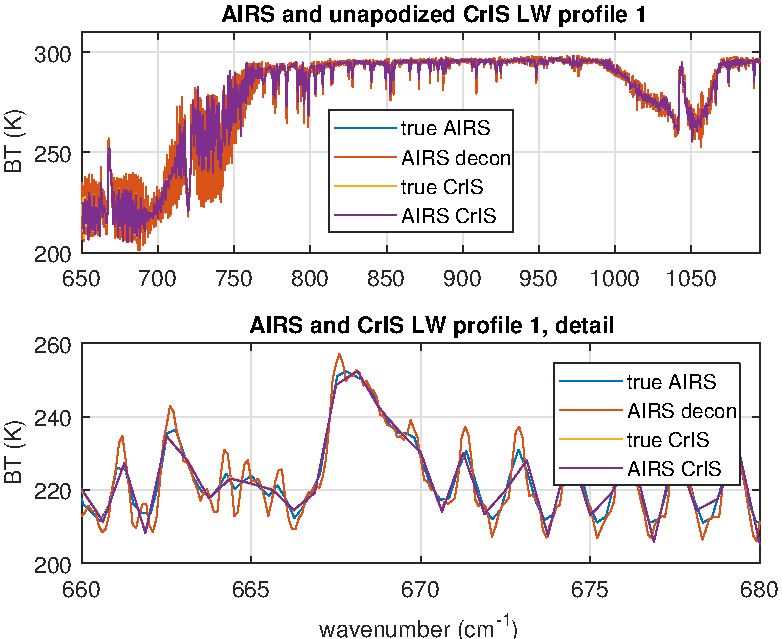
\includegraphics[height=8cm]{figures/a2cris_spec_LW.pdf}
  \caption{true {\cris}, true {\airs}, deconvolved {\airs}, and
    {\airs} {\cris} }
  \label{aclws}
\end{figure}

\begin{figure}
  \centering
  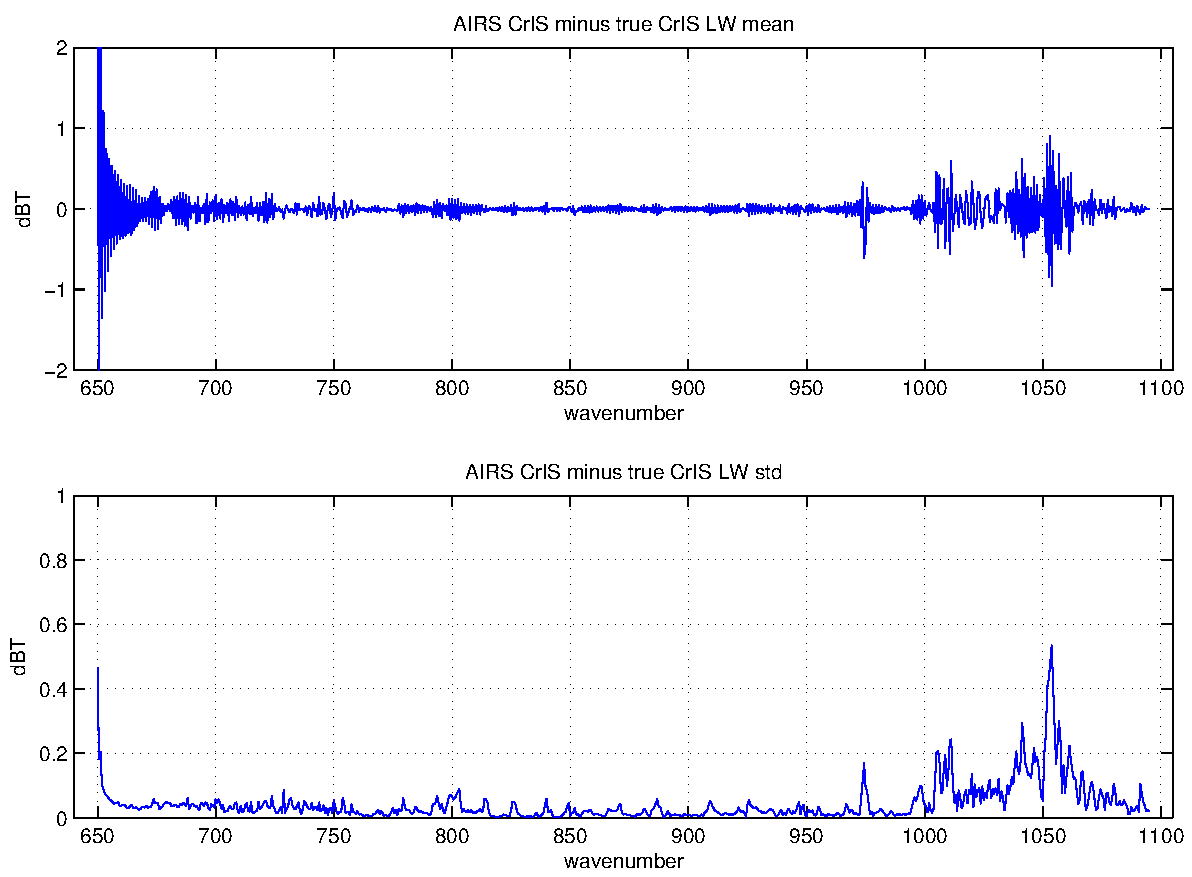
\includegraphics[height=8cm]{figures/airs_cris_diff_LW_noap.pdf}
  \caption{Mean and standard deviation of unapodized {\airs} {\cris}
    minus true {\cris}, for the {\cris} LW band }
  \label{aclwd}
\end{figure}

\begin{figure}
  \centering
  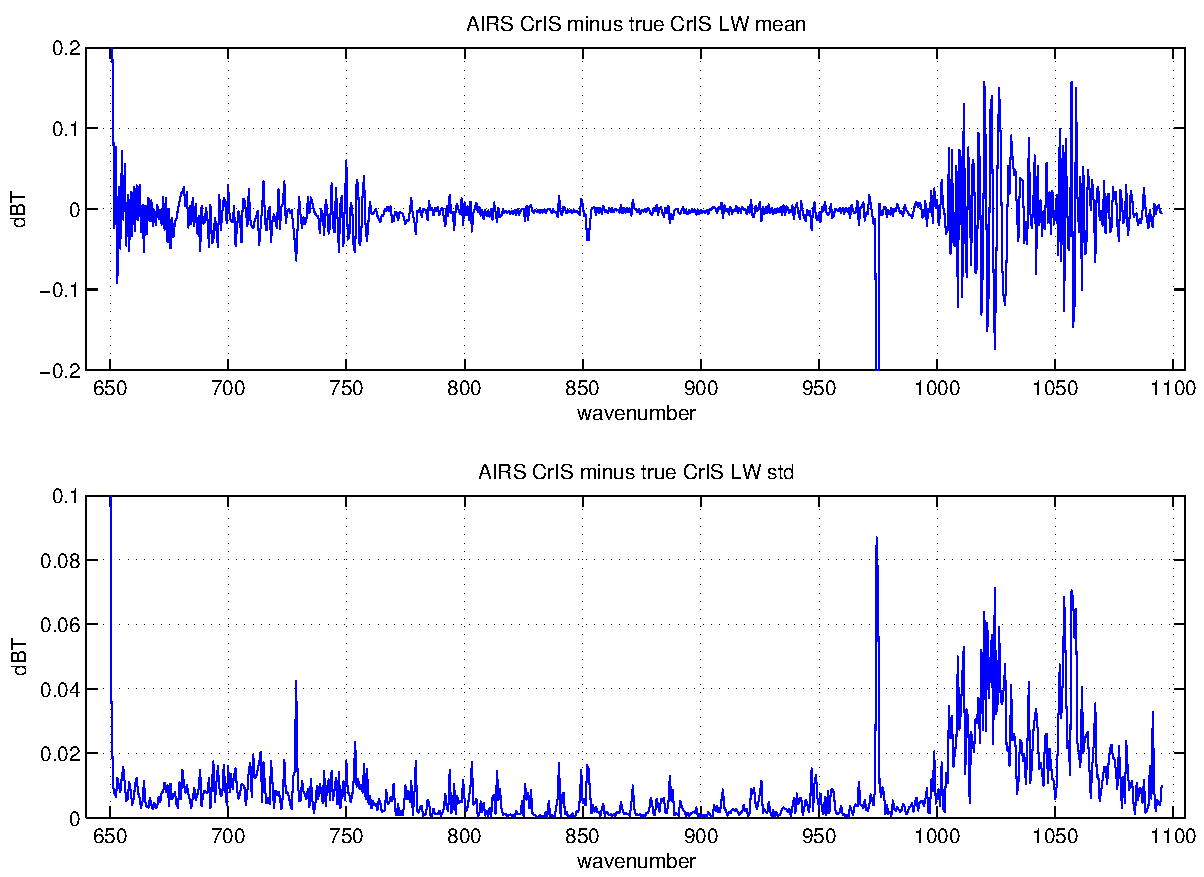
\includegraphics[height=8cm]{figures/airs_cris_diff_LW_hamm.pdf}
  \caption{Mean and standard deviation of Hamming apodized {\airs}
      {\cris} minus true {\cris}, for the {\cris} LW band }
  \label{aclwdh}
\end{figure}

\begin{figure}
  \centering
  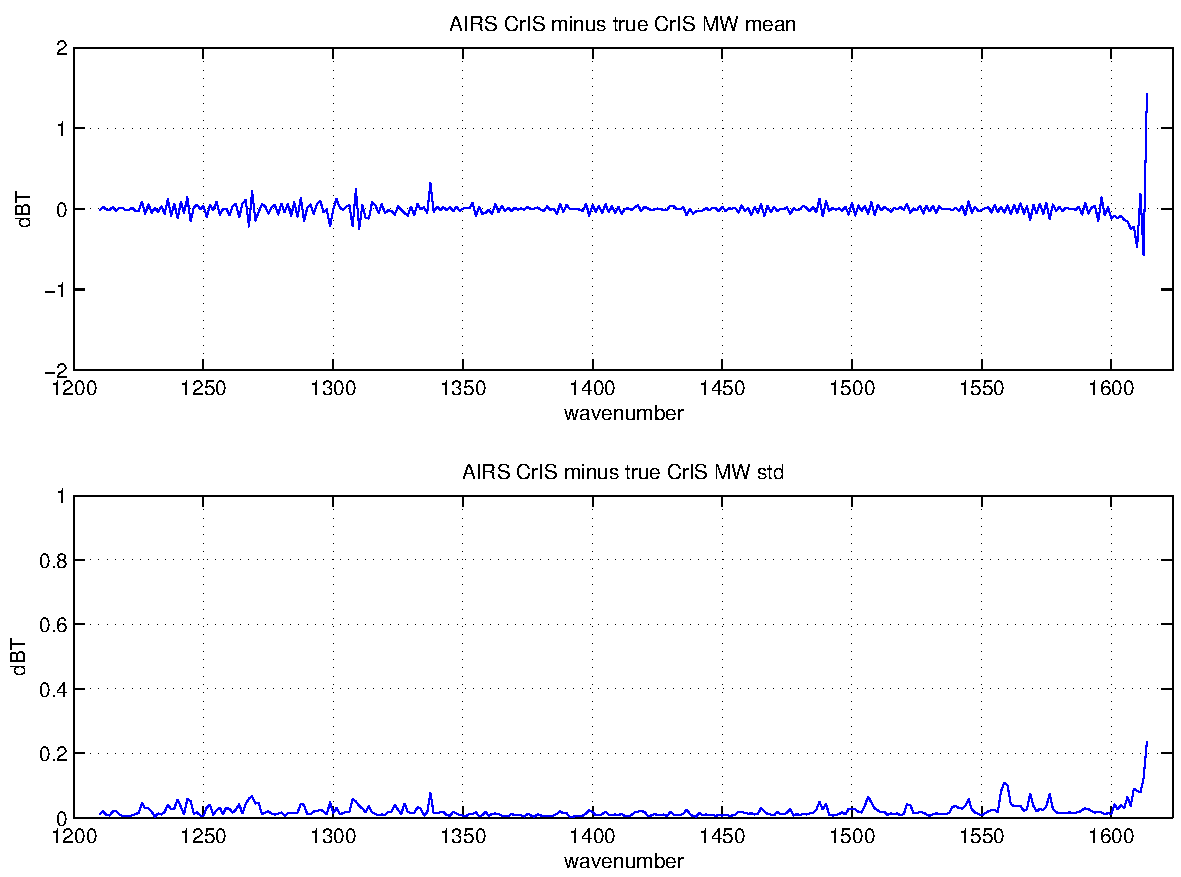
\includegraphics[height=8cm]{figures/airs_cris_diff_MW_noap.pdf}
  \caption{Mean and standard deviation of unapodized {\airs} {\cris}
    minus true {\cris}, for the {\cris} MW band }
  \label{acmwd}
\end{figure}

\begin{figure}
  \centering
  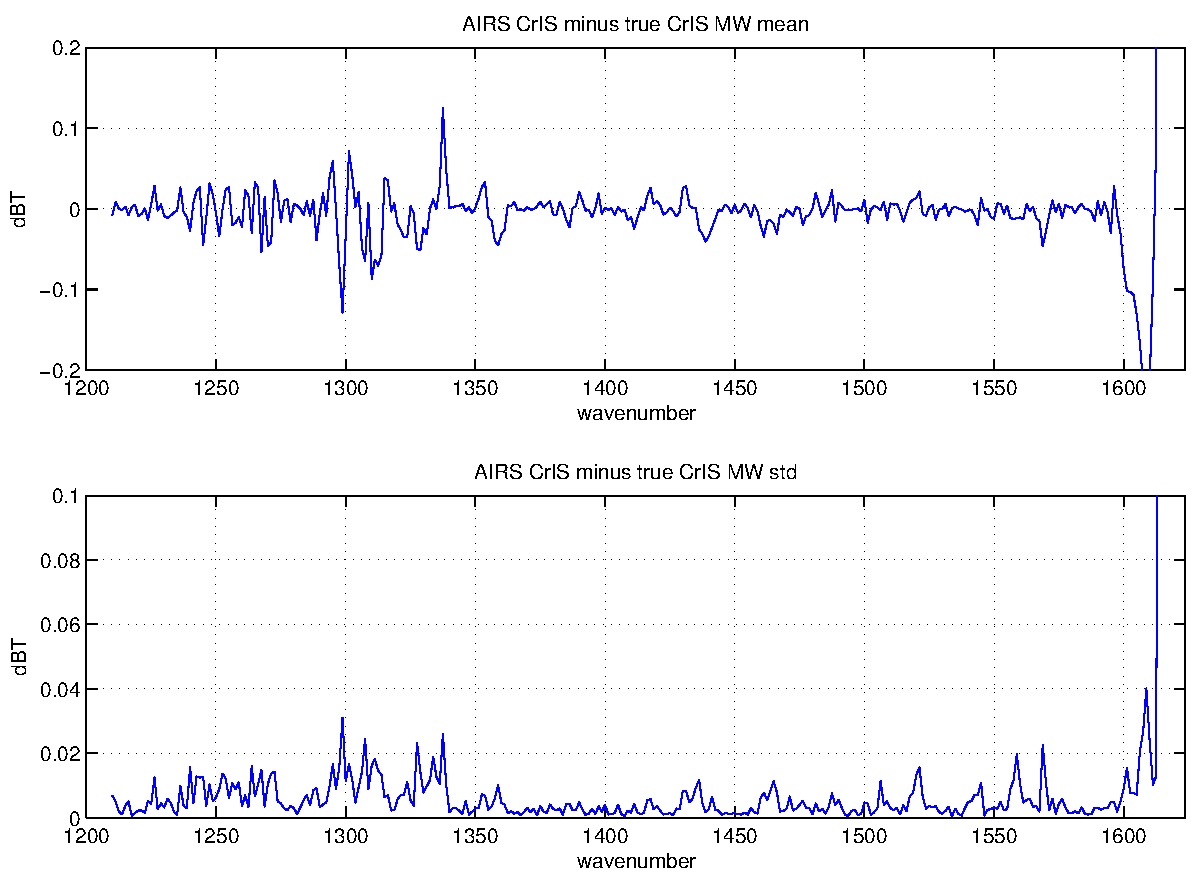
\includegraphics[height=8cm]{figures/airs_cris_diff_MW_hamm.pdf}
  \caption{Mean and standard deviation of Hamming apodized {\airs}
      {\cris} minus true {\cris}, for the {\cris} MW band }
  \label{acmwdh}
\end{figure}

\begin{figure}
  \centering
  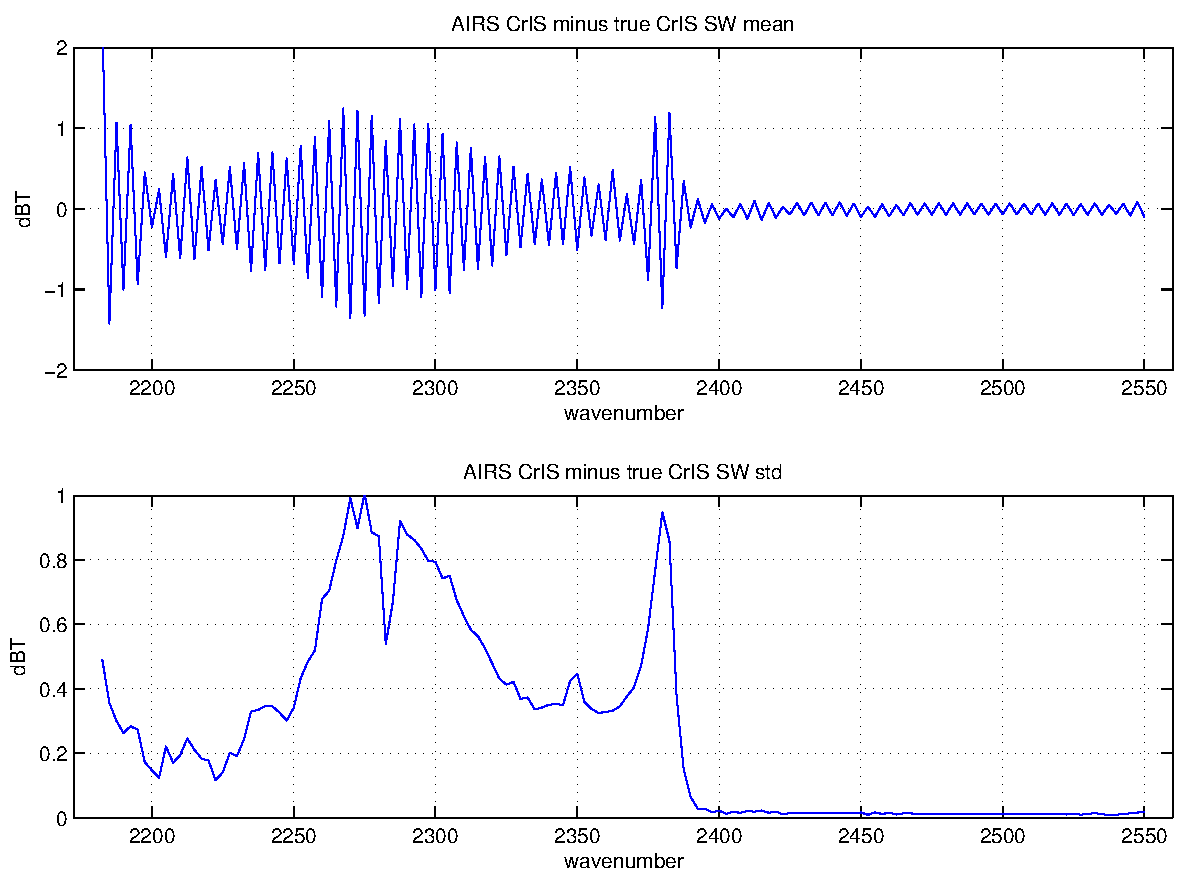
\includegraphics[height=8cm]{figures/airs_cris_diff_SW_noap.pdf}
  \caption{Mean and standard deviation of unapodized {\airs} {\cris}
    minus true {\cris}, for the {\cris} SW band }
  \label{acswd}
\end{figure}

\begin{figure}
  \centering
  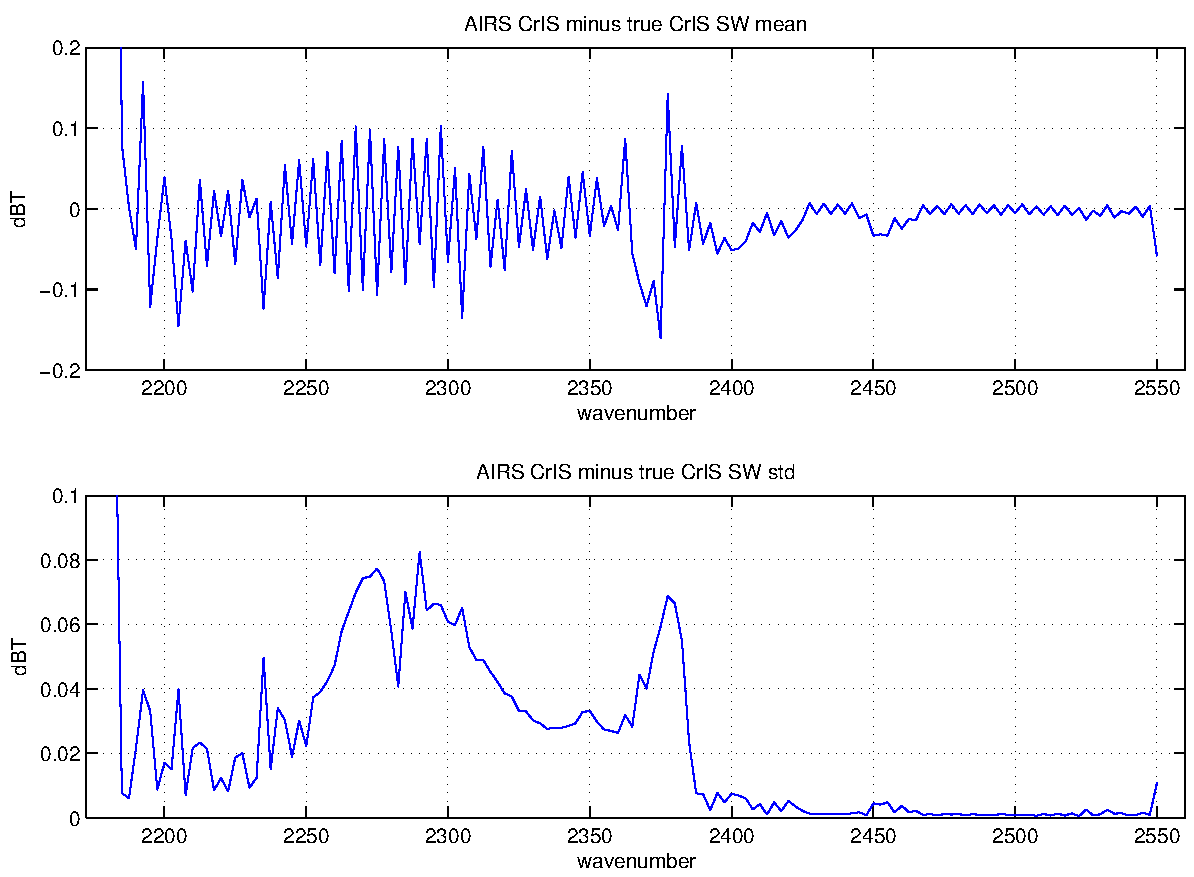
\includegraphics[height=8cm]{figures/airs_cris_diff_SW_hamm.pdf}
  \caption{Mean and standard deviation of Hamming apodized {\airs}
      {\cris} minus true {\cris}, for the {\cris} SW band }
  \label{acswdh}
\end{figure}

For the {\airs} to {\cris} translation deconvolution works better
than both simple interpolation and interpolation (rather than
deconvolution) to an intermediate grid followed by convolution to
{\cris} radiances.  For the first case we start with true {\airs} and
interpolate radiances directly to the {\cris} user grid with a cubic
spline.  For the second we interpolate true {\airs} to the 0.1 {\wn}
intermediate grid with a cubic spline and then convolve this to the
use {\cris} user grid.

\begin{figure}
  \centering
  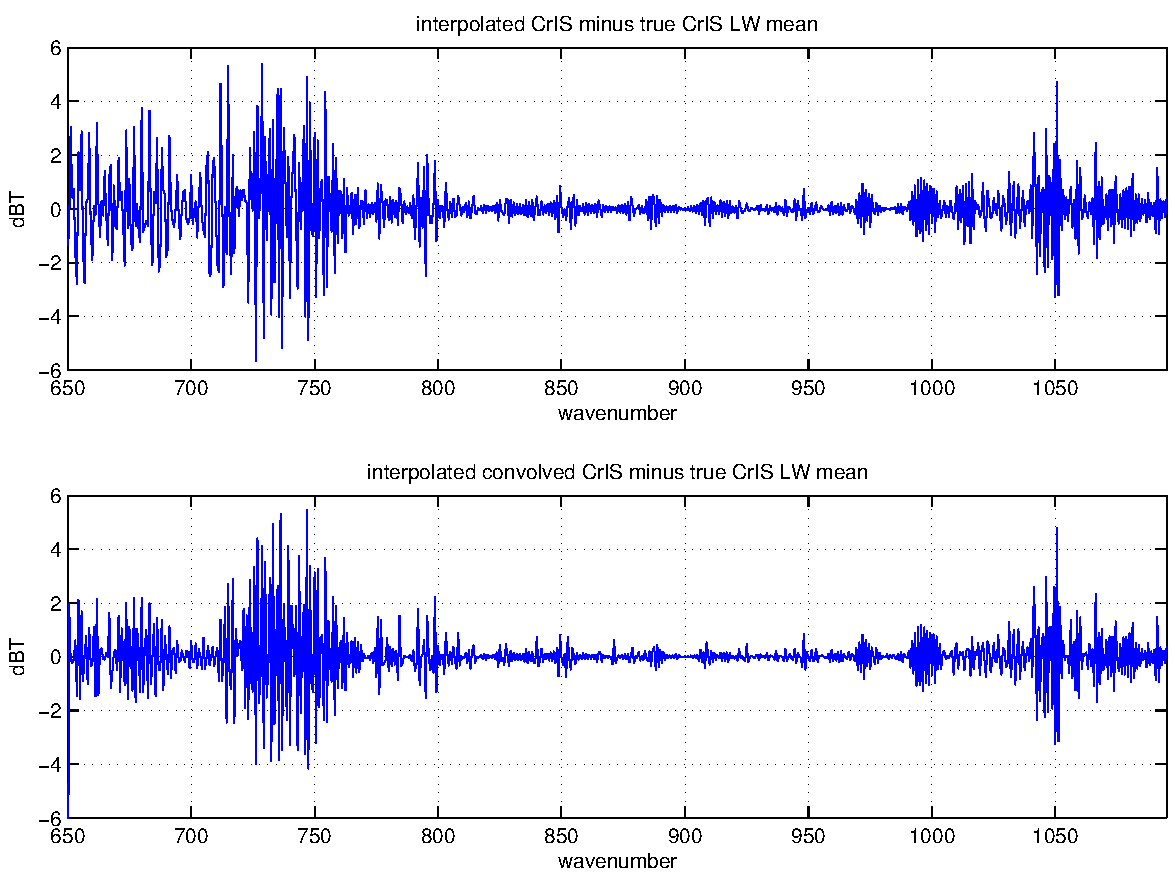
\includegraphics[height=8cm]{figures/airs_cris_intp_LW.pdf}
  \caption{simple interpolation and interpolation with convolution, 
    for the {\cris} LW band}
  \label{intpLW}
\end{figure}

\begin{figure}
  \centering
  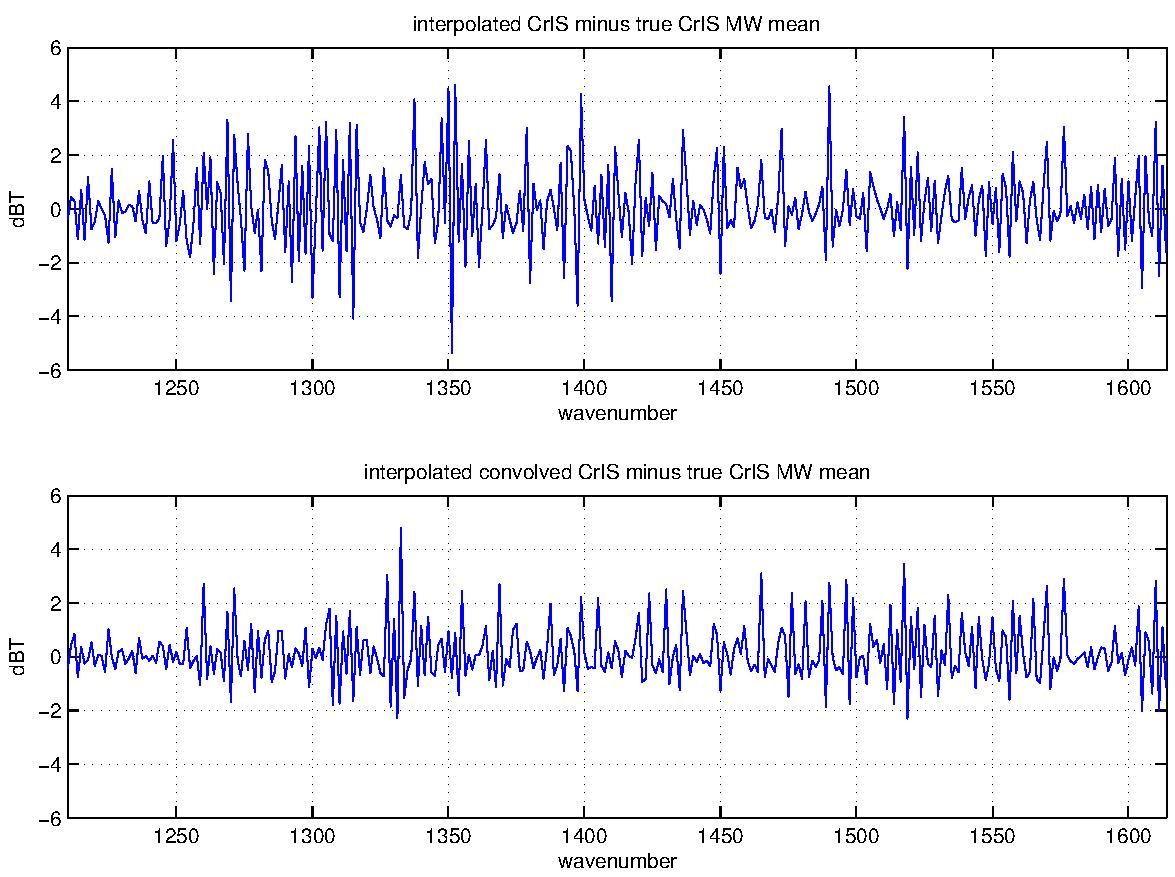
\includegraphics[height=8cm]{figures/airs_cris_intp_MW.pdf}
  \caption{simple interpolation and interpolation with convolution, 
    for the {\cris} MW band}
  \label{intpMW}
\end{figure}

\begin{figure}
  \centering
  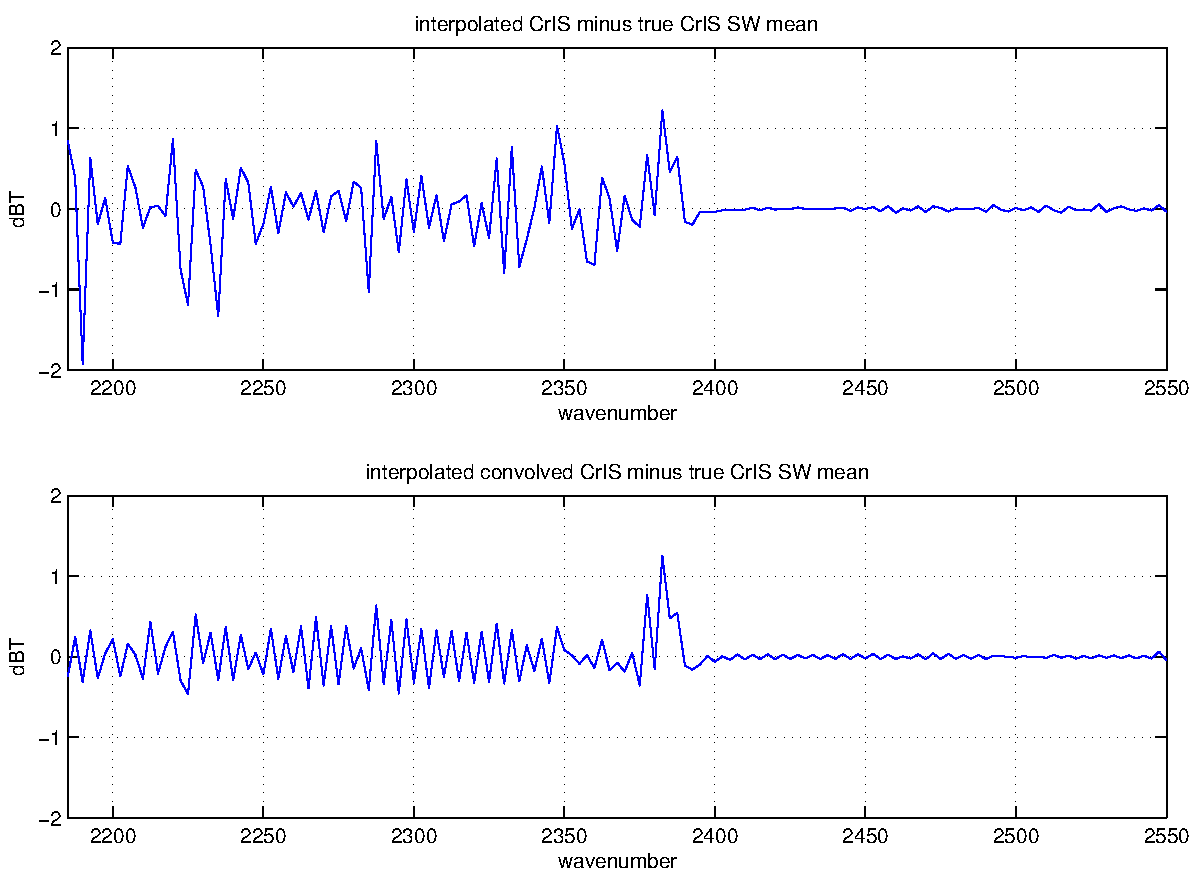
\includegraphics[height=8cm]{figures/airs_cris_intp_SW.pdf}
  \caption{simple interpolation and interpolation with convolution, 
    for the {\cris} SW band}
  \label{intpSW}
\end{figure}

Figure \ref{intpLW} shows interpolated {\cris} minus true {\cris}
for both interpolation tests for the LW band, without any
apodization.  While the two-step interpolation works a little better
than the simple spline, both residuals are significantly larger than
for the translation with deconvolution shown in figure \ref{aclwd}.
Figures \ref{intpMW} and \ref{intpSW} show similar results for the
MW and SW bands.  Deconvolution is significantly better for the MW,
(figure \ref{acmwd}) while the comparison is less clear for the SW
(figure \ref{acswd}).  Comparisons with Hamming apodization show the
residuals with deconvolution are significantly less for all three
bands.

\FloatBarrier
\bibliographystyle{abbrv}
\bibliography{decon}

\end{document}

